%!TEX program = xelatex
\documentclass[times,namecite]{goose-article}

\title{%
  GooseMaterial/AmorphousSolid/LinearStrain/ElastoPlastic
}

\author{T.W.J.~de~Geus}

\contact{%
  $^*$Contact: %
  \href{mailto:tom@geus.me}{tom@geus.me} %
  \hspace{1mm}--\hspace{1mm} %
  \href{http://www.geus.me}{www.geus.me}%
  \hspace{1mm}--\hspace{1mm} %
  \href{https://github.com/tdegeus/GooseMaterial}{https://github.com/tdegeus/GooseMaterial}%
}

\hypersetup{pdfauthor={T.W.J. de Geus}}

\header{%
  \href{https://github.com/tdegeus/GooseMaterial}{GooseMaterial/AmorphousSolid/LinearStrain/ElastoPlastic} -- \href{http://www.geus.me}{T.W.J.\ de Geus}%
}

\newcommand\leftstar[1]{\hspace*{-.3em}~^\star\!#1}

\begin{document}

\maketitle

\begin{abstract}
A microscopic continuum model of plasticity in amorphous solids is proposed. This model uses a strain energy with multiple minima to capture the effect of plasticity. This model is taken from the work of \citet{Jagla2017}.
\end{abstract}

\keywords{elasto-plasticity; linear elasticity}

\setcounter{tocdepth}{2}
\tableofcontents

\vfill\newpage
\section{Constitutive model}

We consider a strain energy $W$ which is composed of two parts, a volumetric (or hydrostatic) part $U$ related to the hydrostatic strain $\varepsilon_\mathrm{m}$, and a shear (or deviatoric ) part $V$ related to the equivalent strain $\varepsilon_\mathrm{eq}$, i.e.\
\begin{equation}
  W ( \bm{\varepsilon} ) = U ( \varepsilon_\mathrm{m} ) + V ( \varepsilon_\mathrm{eq} )
\end{equation}
Our nomenclature can be found in Appendix~\ref{sec:nomenclature} and the definition of the strain measures in Appendix~\ref{sec:strain}. The stress response $\bm{\sigma}$ is the derivative of this energy with respect to the strain tensor $\bm{\varepsilon}$. Before specializing $U$ and $V$ we can already say that
\begin{equation}
  \bm{\sigma}
  =
  \frac{\partial W}{\partial \bm{\varepsilon}}
  =
  \frac{\partial U}{\partial \varepsilon_\mathrm{m}} \;
  \frac{\partial \varepsilon_\mathrm{m}}{\partial \bm{\varepsilon}}
  +
  \frac{\partial V}{\partial \varepsilon_\mathrm{eq}} \;
  \frac{\partial \varepsilon_\mathrm{eq}}{\partial \bm{\varepsilon}}
  =
  \frac{\partial U}{\partial \varepsilon_\mathrm{m}} \;
  \frac{1}{3} \bm{I}
  +
  \frac{\partial V}{\partial \varepsilon_\mathrm{eq}} \;
  \frac{2}{3}
  \frac{\bm{\varepsilon}_d}{\varepsilon_\mathrm{eq}}
\end{equation}
From which we can identity the hydrostatic stress (see Appendix~\ref{sec:stress})
\begin{equation}
  \sigma_\mathrm{m} = \frac{1}{3} \frac{\partial U}{\partial \varepsilon_\mathrm{m}}
\end{equation}
and the deviatoric stress tensor
\begin{equation}
  \bm{\sigma}_\mathrm{d}
  =
  \frac{\partial V}{\partial \varepsilon_\mathrm{eq}} \;
  \frac{2}{3}
  \frac{\bm{\varepsilon}_d}{\varepsilon_\mathrm{eq}}
\end{equation}
From the latter it follows that the equivalent stress
\begin{equation}\label{eq:sig_eq}
  \sigma_\mathrm{eq}
  =
  \sqrt{ \tfrac{3}{2} \bm{\sigma}_\mathrm{d} : \bm{\sigma}_\mathrm{d} }
  =
  \left| \frac{\partial V}{\partial \varepsilon_\mathrm{eq}} \right|
\end{equation}

\subsection{Linear elasticity}

We start simple by considering linear elasticity. In this case the volumetric strain energy $U$ and the shear strain energy $V$ read
\begin{equation}\label{eq:U}
  U ( \varepsilon_\mathrm{m}  ) = \frac{9}{2} \, K \, \varepsilon_\mathrm{m}^2
\end{equation}
and
\begin{equation}\label{eq:V-elas}
  V ( \varepsilon_\mathrm{eq} ) = \frac{3}{2} \, G \, \varepsilon_\mathrm{eq}^2
\end{equation}
The two potentials are plotted in Fig.~\ref{fig:W-elas} (in which we show only $\varepsilon_\mathrm{eq} \geq 0$, as it is by definition non-negative). It is trivial to obtain that
\begin{equation}
  \frac{\partial U}{\partial \varepsilon_\mathrm{m}}
  =
  9 \, K \, \varepsilon_\mathrm{m}
\end{equation}
and
\begin{equation}
  \frac{\partial V}{\partial \varepsilon_\mathrm{eq}}
  =
  3 \, G \, \varepsilon_\mathrm{eq}
\end{equation}
Which corresponds to the well known expression for the stress
\begin{equation}\label{eq:sig-elas}
  \bm{\sigma} ( \bm{\varepsilon} )
  =
  3 K \, \varepsilon_\mathrm{m} \, \bm{I}
  +
  2 G \, \bm{\varepsilon}_\mathrm{d}
\end{equation}
Note that it is also quite common to express Eq.~\eqref{eq:sig-elas} as follows
\begin{equation}
  \bm{\sigma} = \mathbb{C} : \bm{\varepsilon}
\end{equation}
where $\mathbb{C}$ is the fourth-order the elastic stiffness tensor, defined as
\begin{equation}
  \mathbb{C} = K \, \bm{I} \otimes \bm{I} + 2 G \, \mathbb{I}_\mathrm{d}
\end{equation}

\begin{figure}[htp]
  \centering
  \captionsetup[subfigure]{justification=centering}
  \begin{minipage}[t]{.49\textwidth}
    \centering
    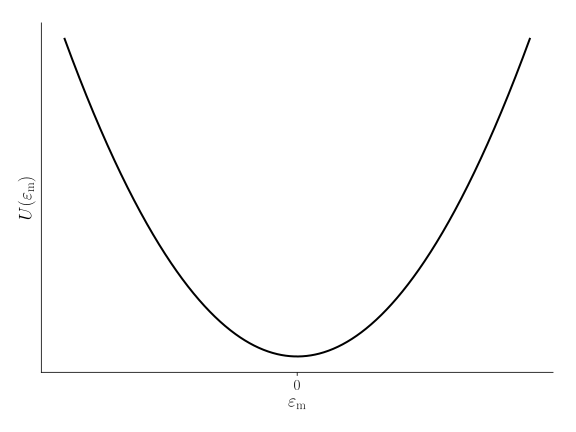
\includegraphics[width=1.\textwidth]{figures/potential_U}
    \subcaption{Volumetric strain energy, $U ( \varepsilon_\mathrm{m} )$}
    \label{fig:U}
  \end{minipage}
  \hfill
  \begin{minipage}[t]{.49\textwidth}
    \centering
    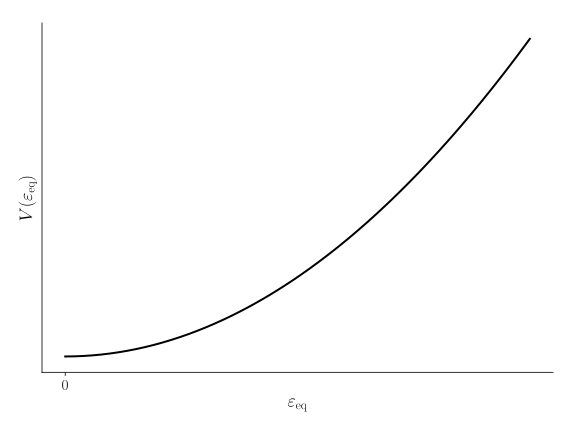
\includegraphics[width=1.\textwidth]{figures/potential_V-elas}
    \subcaption{Shear strain energy, $V ( \varepsilon_\mathrm{eq} )$}
    \label{fig:V-elas}
  \end{minipage}
  \caption{Strain energy $W ( \bm{\varepsilon} ) = U ( \varepsilon_\mathrm{m} ) + V ( \varepsilon_\mathrm{eq} )$ for linear elasticity.}
  \label{fig:W-elas}
\end{figure}

\subsection{Plastic potential}

We now extend the model to account for plasticity. For this we strive for a model that is volumetrically purely elastic, while in shear, the model is governed by multiple minima. These minima have the effect that when the material reaches a certain yield stress it jumps to the next minimum. Around this minimum the elasticity is always the same. When loading is continued the the material again jumps to a new minimum when the next yield stress is reached. The magnitudes of the jumps and of the yield stress are thereby related.

\begin{figure}[htp]
  \centering
  \captionsetup[subfigure]{justification=centering}
  \begin{minipage}[t]{.49\textwidth}
    \centering
    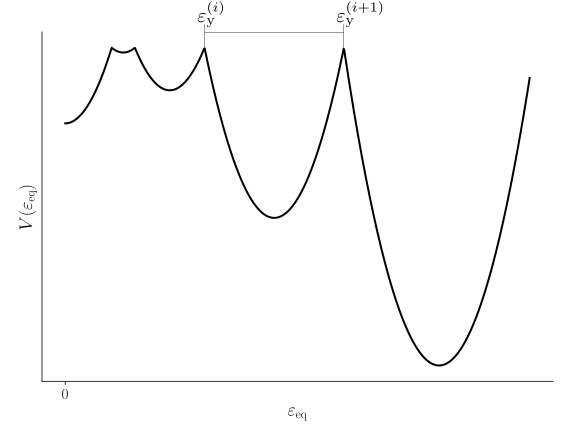
\includegraphics[width=1.\textwidth]{figures/potential_V-plas}
    \subcaption{Multi-parabolic shear strain energy}
    \label{fig:V-plas}
  \end{minipage}
  \hfill
  \begin{minipage}[t]{.49\textwidth}
    \centering
    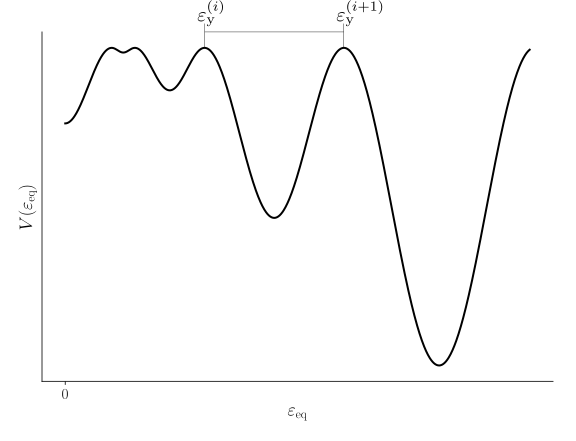
\includegraphics[width=1.\textwidth]{figures/potential_V-plas-smooth}
    \subcaption{Smooth multi-parabolic shear strain energy}
    \label{fig:V-plas-smooth}
  \end{minipage}
  \caption{The multi-minima shear strain energy, $V ( \varepsilon_\mathrm{eq} )$, that models the effect of plasticity. The multi-parabolic shear strain energy is shown in (a), while its smoothened equivalent is shown in (b).}
\end{figure}

\paragraph{Parabolic potential with multiple minima}

As described, the volumetric behavior is give by Eq.~\eqref{eq:U} and plotted in Fig.~\ref{fig:U}. To attain the desired behavior in shear we divide the equivalent strain space in a finite number of yield strains $\varepsilon_\mathrm{y}^{(0)}, \varepsilon_\mathrm{y}^{(1)}, \varepsilon_\mathrm{y}^{(2)}, ...$ and define a parabolic potential between each pair ($[ \varepsilon_\mathrm{y}^{(0)}, \varepsilon_\mathrm{y}^{(1)} )$, $[ \varepsilon_\mathrm{y}^{(1)}, \varepsilon_\mathrm{y}^{(2)} )$, ...). The shear strain energy is then composed of a manifold of quadratic contributions
\begin{equation}\label{eq:V-plas}
  V \big(
    \varepsilon_\mathrm{y}^{(i)} \leq \varepsilon_\mathrm{eq} < \varepsilon_\mathrm{y}^{(i+1)}
  \big)
  =
  V^{(i)}
  =
  \frac{3}{2} \, G \, \bigg[\,
    \Big[\, \varepsilon_\mathrm{eq} - \varepsilon_\mathrm{min}^{(i)} \,\Big]^2
    -
    \Big[\, \Delta \varepsilon_\mathrm{y}^{(i)} \,\Big]^2
  \,\bigg]
\end{equation}
where the mean of $\varepsilon_\mathrm{y}^{(i)}$ and $\varepsilon_\mathrm{y}^{(i+1)}$ is
\begin{equation}
  \varepsilon_\mathrm{min}^{(i)}
  =
  \frac{1}{2} \Big[\, \varepsilon_\mathrm{y}^{(i+1)} + \varepsilon_\mathrm{y}^{(i)} \,\Big]
\end{equation}
which is also the equivalent strain at which the shear strain energy reaches its minimum; and the distance to $\varepsilon_\mathrm{y}^{(i)}$ and $\varepsilon_\mathrm{y}^{(i+1)}$ is
\begin{equation}
  \Delta \varepsilon_\mathrm{y}^{(i)}
  =
  \frac{1}{2} \Big[\, \varepsilon_\mathrm{y}^{(i+1)} - \varepsilon_\mathrm{y}^{(i)} \,\Big]
\end{equation}
The resulting shear strain energy is plotted in Fig.~\ref{fig:V-plas}

To compute the stress we need
\begin{equation}\label{eq:dV-plas}
  \frac{\partial V^{(i)}}{\partial \varepsilon_\mathrm{eq}}
  =
  3 \, G \, \Big[\, \varepsilon_\mathrm{eq} - \varepsilon_\mathrm{min}^{(i)} \,\Big]
\end{equation}
For which we can observe that around $\varepsilon_\mathrm{min}^{(i)}$ the elastic response is similar to linear elasticity. If we take $\varepsilon_\mathrm{y}^{(0)} = - \varepsilon_\mathrm{y}^{(1)}$ we even find exactly linear elasticity until the initial yield stress is reached. For completeness, the stress reads
\begin{equation}
  \bm{\sigma} ( \bm{\varepsilon} )
  =
  3 K \, \varepsilon_\mathrm{m} \, \bm{I}
  +
  2 \, G \, \Big[\, 1 - \varepsilon_\mathrm{min}^{(i)} / \varepsilon_\mathrm{eq} \,\Big] \;
  \bm{\varepsilon}_\mathrm{d}
  \qquad
  \mathrm{for}
  \qquad
  \varepsilon_\mathrm{y}^{(i)} \leq \varepsilon_\mathrm{eq} < \varepsilon_\mathrm{y}^{(i+1)}
\end{equation}
whereby we make the assumption that when $\varepsilon_\mathrm{eq} = 0$ also $\bm{\sigma}_\mathrm{d} = \bm{0}$ in order to avoid zero-devision.

\paragraph{Smooth parabolic potential with multiple minima}

Next to this we also define a smoothened equivalent of Eq.~\eqref{eq:V-plas}:
\begin{equation}\label{eq:V-plas-smooth}
  V \big(
    \varepsilon_\mathrm{y}^{(i)} \leq \varepsilon_\mathrm{eq} < \varepsilon_\mathrm{y}^{(i+1)}
  \big)
  =
  V^{(i)}
  =
  - 3 \, G \,
  \left[ \frac{\Delta \varepsilon_\mathrm{y}^{(i)}}{\pi} \right]^2
  \left[
    1
    +
    \cos \left(
      \frac{ \pi }{ \Delta \varepsilon_\mathrm{y}^{(i)} }
      \Big[\, \varepsilon_\mathrm{eq} - \varepsilon_\mathrm{min}^{(i)} \,\Big]
    \right)
  \right]
\end{equation}
which is plotted in Fig.~\ref{fig:V-plas-smooth}. In this case we obtain
\begin{equation}\label{eq:dV-plas-smooth}
  \frac{\partial V^{(i)}}{\partial \varepsilon_\mathrm{eq}}
  =
  3 \, G \,
  \left[ \frac{\Delta \varepsilon_\mathrm{y}^{(i)}}{\pi} \right]
  \sin \left(
    \frac{ \pi }{ \Delta \varepsilon_\mathrm{y}^{(i)} }
    \Big[\, \varepsilon_\mathrm{eq} - \varepsilon_\mathrm{min}^{(i)} \,\Big]
  \right)
\end{equation}
Which is to the first order equal to linear elasticity around its minimum $\varepsilon_\mathrm{min}^{(i)}$. Indeed, the first order Taylor series of Eq.~\eqref{eq:dV-plas-smooth} around $\varepsilon_\mathrm{eq} = \varepsilon_\mathrm{min}^{(i)}$,
\begin{equation}
  \frac{\partial V^{(i)}}{\partial \varepsilon_\mathrm{eq}}
  \approx
  3 \, G \, \Big[\, \varepsilon_\mathrm{eq} - \varepsilon_\mathrm{min}^{(i)} \,\Big]
\end{equation}
is identical to Eq.~\eqref{eq:dV-plas}.

For completeness also in case the stress tensor
\begin{equation}
  \bm{\sigma} ( \bm{\varepsilon} )
  =
  3 K \, \varepsilon_\mathrm{m} \, \bm{I}
  +
  2 \, G \,
  \left[ \frac{\Delta \varepsilon_\mathrm{y}^{(i)}}{\pi} \right]
  \sin \left(
    \frac{ \pi }{ \Delta \varepsilon_\mathrm{y}^{(i)} }
    \Big[\, \varepsilon_\mathrm{eq} - \varepsilon_\mathrm{min}^{(i)} \,\Big]
  \right)
  \frac{\bm{\varepsilon}_\mathrm{d}}{\varepsilon_\mathrm{eq}}
  \qquad
  \mathrm{for}
  \qquad
  \varepsilon_\mathrm{y}^{(i)} \leq \varepsilon_\mathrm{eq} < \varepsilon_\mathrm{y}^{(i+1)}
\end{equation}
whereby we again make the assumption that when $\varepsilon_\mathrm{eq} = 0$ also $\bm{\sigma}_\mathrm{d} = \bm{0}$.

\section{Stress response}

We next investigate the stress response for a monotonically increasing $\varepsilon_\mathrm{eq}$. The idea is to get a feeling for the behavior of a material. But one must realize that for a specimen the stress response is determined from mechanical equilibrium, which implies that the material's response is also determined from it's surroundings. A typical macroscopic stress--strain curves will look quite different to what is presented here.

To obtain the stress response we start from the derivative of the shear strain energy, Eqs.~(\ref{eq:dV-plas},\ref{eq:dV-plas-smooth}). These are plotted in Fig.~\ref{fig:dV-plas}. The equivalent stress $\sigma_\mathrm{eq}$ can now be obtained using Eq.~\eqref{eq:sig_eq}; the result of which is plotted in Fig.~\ref{fig:sigeq-plas}.

\begin{figure}[htp]
  \centering
  \captionsetup[subfigure]{justification=centering}
  \begin{minipage}[t]{.49\textwidth}
    \centering
    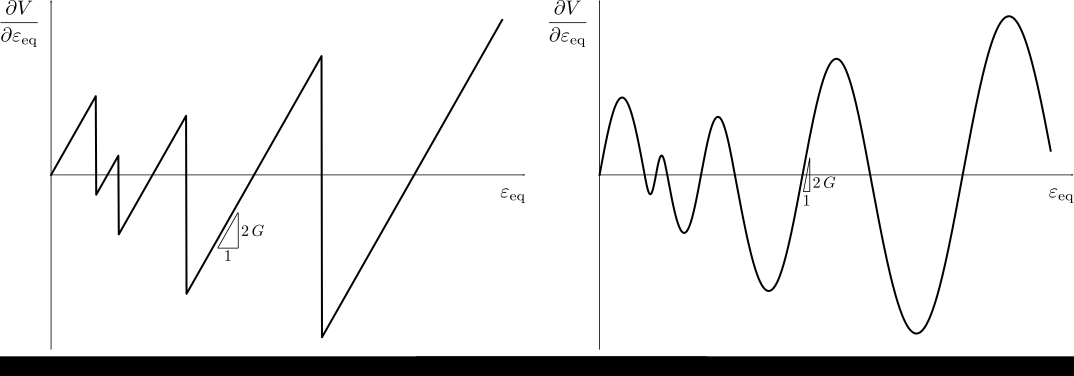
\includegraphics[width=1.\textwidth]{figures/potential_dV-plas}
    \subcaption{Multi-parabolic shear strain energy}
  \end{minipage}
  \hfill
  \begin{minipage}[t]{.49\textwidth}
    \centering
    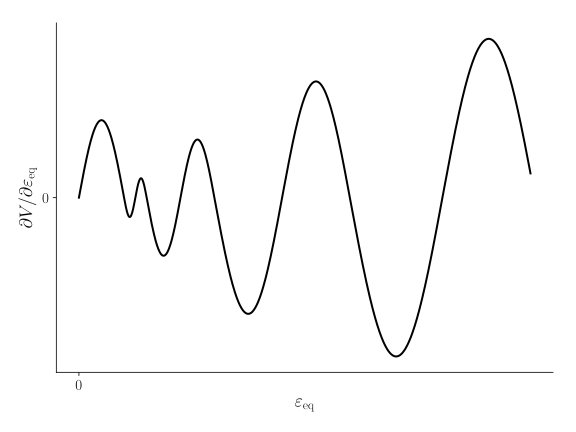
\includegraphics[width=1.\textwidth]{figures/potential_dV-plas-smooth}
    \subcaption{Smooth multi-parabolic shear strain energy}
  \end{minipage}
  \caption{Derivate of the shear strain energy $V$.}
  \label{fig:dV-plas}
\end{figure}

\begin{figure}[htp]
  \centering
  \captionsetup[subfigure]{justification=centering}
  \begin{minipage}[t]{.49\textwidth}
    \centering
    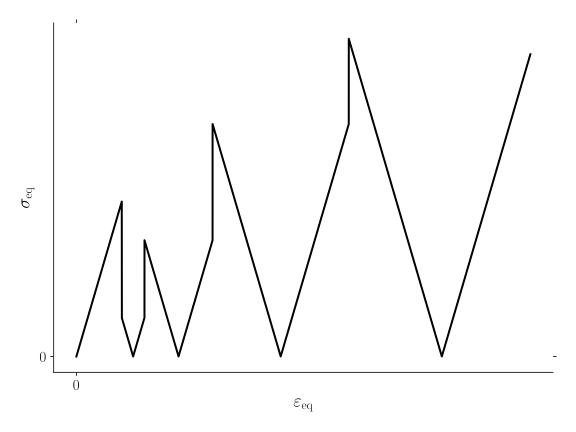
\includegraphics[width=1.\textwidth]{figures/stress-strain}
    \subcaption{Multi-parabolic shear strain energy}
  \end{minipage}
  \hfill
  \begin{minipage}[t]{.49\textwidth}
    \centering
    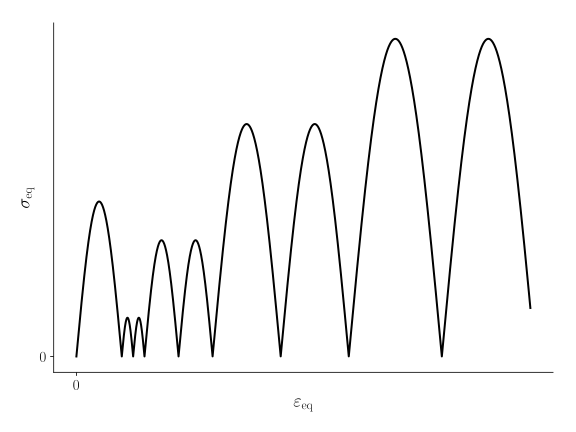
\includegraphics[width=1.\textwidth]{figures/stress-strain-smooth}
    \subcaption{Smooth multi-parabolic shear strain energy}
  \end{minipage}
  \caption{Stress--strain response. The equivalent (shear) stress $\sigma_\mathrm{eq}$ is plotted as a function of the equivalent strain $\varepsilon_\mathrm{eq}$ for both the multi-parabolic shear strain energy and its smoothened equivalent. Although not important for the result here, note that this response is actually obtained from the implementation by applying monotonically increasing simple shear.}
  \label{fig:sigeq-plas}
\end{figure}

\appendix
\vfill\newpage

\section{Nomenclature}
\label{sec:nomenclature}

\begin{itemize}
%
\item Dyadic tensor product
\begin{align}
  \mathbb{C} &= \bm{A} \otimes \bm{B} \\
  C_{ijkl}   &= A_{ij} \,      B_{kl}
\end{align}
%
\item Double tensor contraction
\begin{align}
  C &= \bm{A} : \bm{B} \\
    &= A_{ij} \, B_{ji}
\end{align}
%
\item Deviatoric projection tensor
\begin{equation}
  \mathbb{I}_\mathrm{d}
  = \mathbb{I}_\mathrm{s} - \frac{1}{3} \bm{I} \otimes \bm{I}
\end{equation}
%
\end{itemize}

\section{Strain measures}
\label{sec:strain}

\begin{itemize}
%
\item Mean strain
\begin{equation}
  \varepsilon_\mathrm{m}
  = \tfrac{1}{3} \, \mathrm{tr} ( \bm{\varepsilon} )
  = \tfrac{1}{3} \, \bm{\varepsilon} : \bm{I}
\end{equation}
%
\item Strain deviator
\begin{equation}
  \bm{\varepsilon}_\mathrm{d}
  = \bm{\varepsilon} - \varepsilon_\mathrm{m} \, \bm{I}
  = \mathbb{I}_\mathrm{d} : \bm{\varepsilon}
\end{equation}
%
\item Equivalent strain
\begin{equation}
  \varepsilon_\mathrm{eq}
  = \; \sqrt{
    \tfrac{2}{3} \, \bm{\varepsilon}_\mathrm{d} : \bm{\varepsilon}_\mathrm{d}
  }
\end{equation}
%
\end{itemize}

\section{Stress measures}
\label{sec:stress}

\begin{itemize}
%
\item Mean stress
%
\begin{equation}
\sigma_\mathrm{m}
= \tfrac{1}{3} \, \mathrm{tr} ( \bm{\sigma} )
= \tfrac{1}{3} \, \bm{\sigma} : \bm{I}
\end{equation}
%
\item Stress deviator
%
\begin{equation}
  \bm{\sigma}_\mathrm{d}
  = \bm{\sigma} - \sigma_\mathrm{m} \, \bm{I}
  = \mathbb{I}_\mathrm{d} : \bm{\sigma}
\end{equation}
%
\item Von Mises equivalent stress
\begin{equation}
\sigma_\mathrm{eq} = \sqrt{ \tfrac{3}{2} \, \bm{\sigma}_\mathrm{d} : \bm{\sigma}_\mathrm{d} }
\end{equation}
%
\end{itemize}

\section{Derivatives}
\label{sec:derivatives}

\begin{itemize}
%
\item Strain deviator
\begin{equation}
  \frac{ \partial \bm{\varepsilon}_\mathrm{d} }{ \partial \bm{\varepsilon} }
  = \mathbb{I}_\mathrm{d}
\end{equation}
%
\item Mean equivalent strain
\begin{equation}
  \frac{ \partial \varepsilon_\mathrm{m} }{ \partial \bm{\varepsilon} }
  =
  \frac{1}{3} \bm{I} : \mathbb{I}
  =
  \frac{1}{3} \bm{I}
\end{equation}
%
\item Von Mises equivalent strain
\begin{equation}
  \frac{ \partial \varepsilon_\mathrm{eq} }{ \partial \bm{\varepsilon} }
  =
  \frac{1}{2 \varepsilon_\mathrm{eq}} \frac{2}{3}
  \big[\, \mathbb{I}_\mathrm{d} : \bm{\varepsilon}_\mathrm{d} + \bm{\varepsilon}_\mathrm{d} : \mathbb{I}_\mathrm{d} \,\big]
  =
  \frac{2}{3} \frac{\bm{\varepsilon}_\mathrm{d}}{\varepsilon_\mathrm{eq}}
\end{equation}
%
\end{itemize}

\bibliography{library}

\end{document}
